\section{Linker}

The final element in the chain of the build process is the linker. It takes the
object files that were produced by the compiler in the previous step and resolves
all symbols in other files.

On a related note, an important term that often appears in this context is the word
linkage. A distinction is drawn between internal and external linkage. Internal
linkage refers to any identifier whose accessibility is limited to a single
translation unit. By contrast, external linkage refers to any identifier that is
accessible by other translation units via a forward declaration.

At first glance it might seem strange to separate the compilation process from
the linker. But there are several advantages to this design:

\begin{itemize}
    \item A modular design enables the compiler to work with different but
    compatible linkers.
    \item The implementation complexity of the compiler is possibly reduced if both
    steps are distinct from each other (e.g., during compilation it can assume that
    a function is defined in another file).
    \item Because the linker springs into action as a post-compilation process,
    modifying a single header file does not necessarily induce the re-compilation
    of all project files (with the exception of any file that includes this header),
    one consequence of which is the fact is that the complete build process takes
    up less time.
    \item This distinction also enables multi-threaded compilation which further
    speeds up the build process.
\end{itemize}

On top of that there are more benefits to this approach. Understanding the difference
between compilation and linking makes it easier to interpret bugs in code. Error
messages often indicate at which stage an error was detected:

\begin{itemize}
    \item \texttt{LNK2019: unresolved external symbol 'symbol' referenced in function 'function'.}
    \item \texttt{C2661: 'function': no overloaded function takes number arguments. }
\end{itemize}

In general, the compiler is capable of generating more precise error messages because
it has access to the abstract syntax tree (or an intermediate code representation
in case of Clang), which is why it can reason better about the code at hand. Therefore,
it is a good idea to write code in a way that any possible errors are caught by
the compiler rather than by the linker.

\begin{figure}[ht]
    \centering
    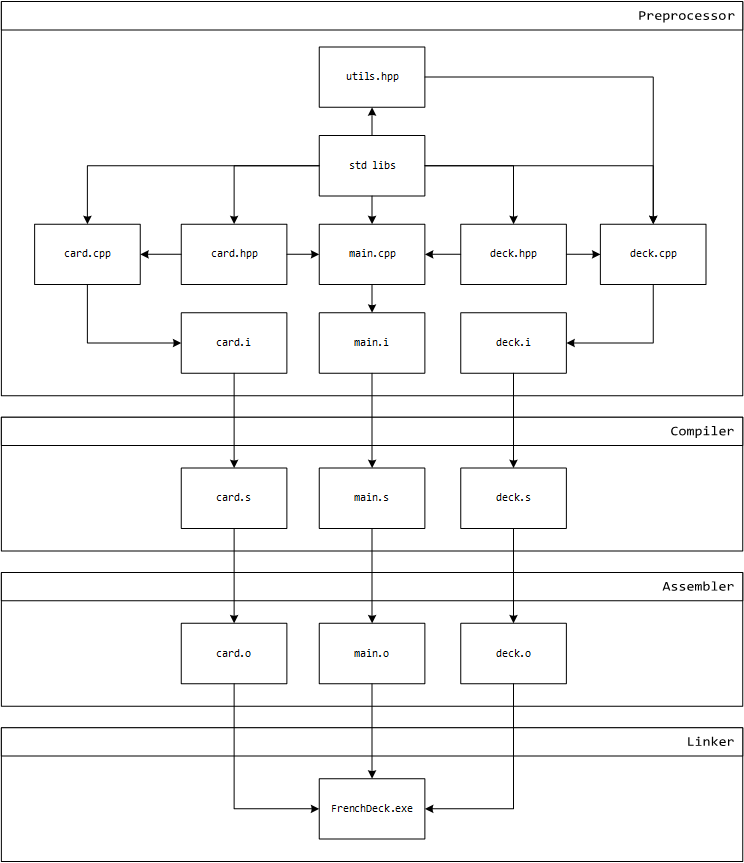
\includegraphics[width=1\textwidth]{images/FrenchDeck.png}
\end{figure}
